\documentclass{standalone}
\usepackage{tikz}
\usetikzlibrary{patterns, positioning}
\usepackage[sfdefault]{ClearSans} %% option 'sfdefault' activates Clear Sans as the default text font
\usepackage[T1]{fontenc}

\begin{document}
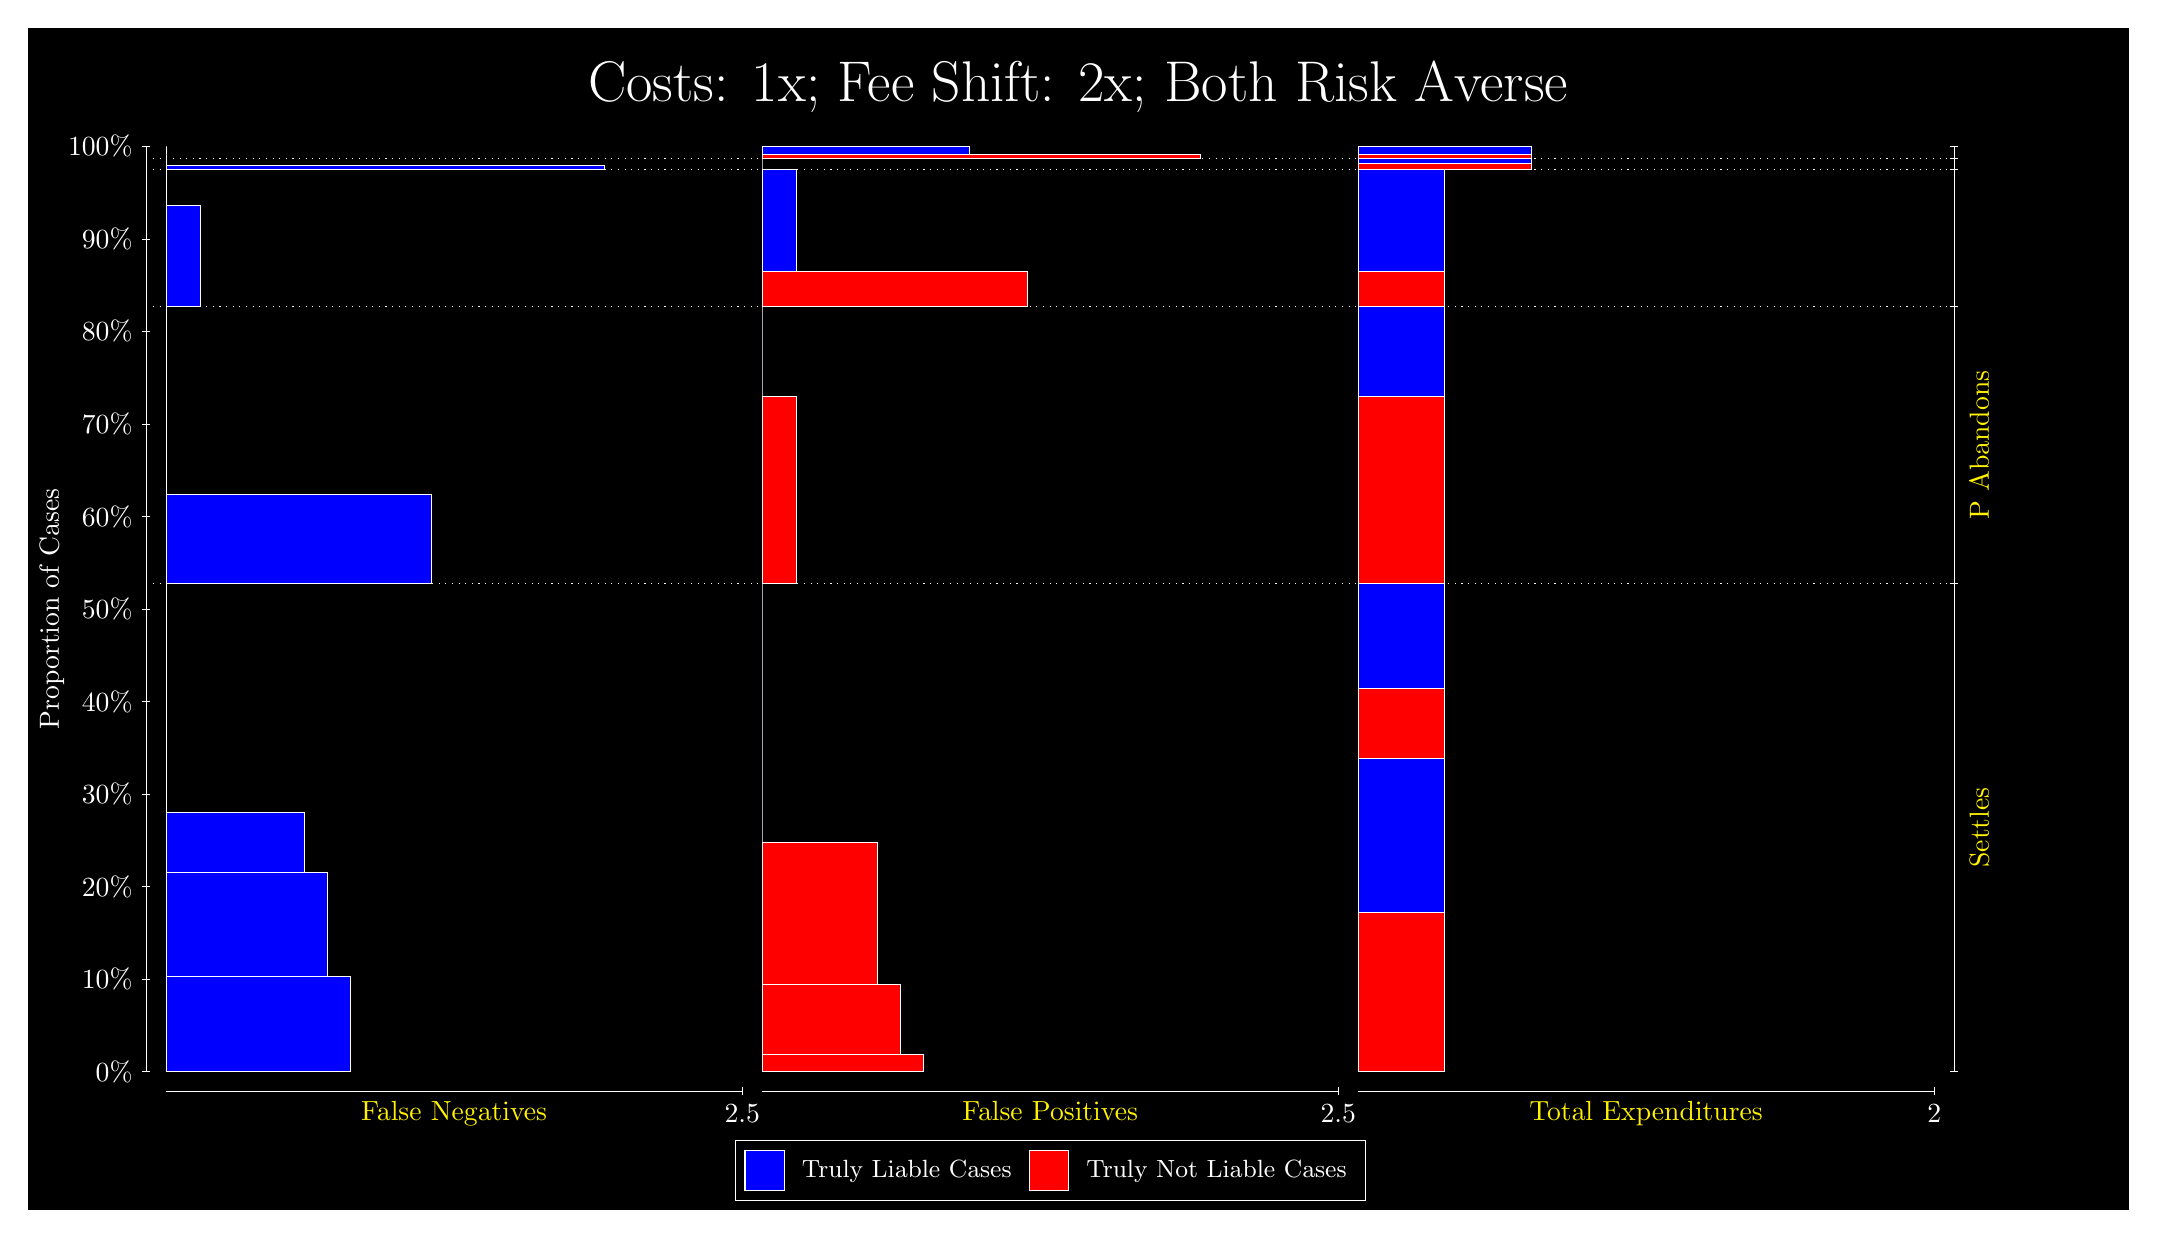
\begin{tikzpicture}
\draw[fill=black] (0,0) rectangle (26.667,15);
\draw[text=white] (0,13.5) rectangle (26.667,15) node[midway] {\huge Costs: 1x; Fee Shift: 2x; Both Risk Averse};
\draw[white, very thin] (1.5,1.75) -- (1.5,13.5);
\node[rotate=90, text=white, anchor=center] at (0.3, 7.625) {Proportion of Cases};
\draw[white, very thin] (1.45,1.75) -- (1.55,1.75);
\node[text=white, anchor=east] at (1.45, 1.75) {0\%};
\draw[white, very thin] (1.45,2.925) -- (1.55,2.925);
\node[text=white, anchor=east] at (1.45, 2.925) {10\%};
\draw[white, very thin] (1.45,4.1) -- (1.55,4.1);
\node[text=white, anchor=east] at (1.45, 4.1) {20\%};
\draw[white, very thin] (1.45,5.275) -- (1.55,5.275);
\node[text=white, anchor=east] at (1.45, 5.275) {30\%};
\draw[white, very thin] (1.45,6.45) -- (1.55,6.45);
\node[text=white, anchor=east] at (1.45, 6.45) {40\%};
\draw[white, very thin] (1.45,7.625) -- (1.55,7.625);
\node[text=white, anchor=east] at (1.45, 7.625) {50\%};
\draw[white, very thin] (1.45,8.8) -- (1.55,8.8);
\node[text=white, anchor=east] at (1.45, 8.8) {60\%};
\draw[white, very thin] (1.45,9.975) -- (1.55,9.975);
\node[text=white, anchor=east] at (1.45, 9.975) {70\%};
\draw[white, very thin] (1.45,11.15) -- (1.55,11.15);
\node[text=white, anchor=east] at (1.45, 11.15) {80\%};
\draw[white, very thin] (1.45,12.325) -- (1.55,12.325);
\node[text=white, anchor=east] at (1.45, 12.325) {90\%};
\draw[white, very thin] (1.45,13.5) -- (1.55,13.5);
\node[text=white, anchor=east] at (1.45, 13.5) {100\%};

\draw[white, very thin] (24.457,1.75) -- (24.457,13.5);
\draw[white, very thin] (24.407,1.75) -- (24.507,1.75);
\node[anchor=west] at (24.407, 1.75) {};
\draw[white, very thin] (24.407,7.9496) -- (24.507,7.9496);
\node[anchor=west] at (24.407, 7.9496) {};
\draw[white, very thin] (24.407,11.466) -- (24.507,11.466);
\node[anchor=west] at (24.407, 11.466) {};
\draw[white, very thin] (24.407,13.207) -- (24.507,13.207);
\node[anchor=west] at (24.407, 13.207) {};
\draw[white, very thin] (24.407,13.346) -- (24.507,13.346);
\node[anchor=west] at (24.407, 13.346) {};
\draw[white, very thin] (24.407,13.5) -- (24.507,13.5);
\node[anchor=west] at (24.407, 13.5) {};

\draw[white, very thin, fill=blue] (1.75,1.75) rectangle (4.092,2.9536);
\draw[white, very thin, fill=blue] (1.75,2.9536) rectangle (3.7993,4.2816);
\draw[white, very thin, fill=blue] (1.75,4.2816) rectangle (3.5065,5.0385);
\draw[white, very thin, fill=red] (1.75,5.0385) rectangle (1.75,7.9496);
\draw[white, very thin, fill=blue] (1.75,7.9496) rectangle (5.1167,9.0864);
\draw[white, very thin, fill=red] (1.75,9.0864) rectangle (1.75,11.466);
\draw[white, very thin, fill=blue] (1.75,11.466) rectangle (2.1891,12.755);
\draw[white, very thin, fill=red] (1.75,12.755) rectangle (1.75,13.207);
\draw[white, very thin, fill=blue] (1.75,13.207) rectangle (7.3123,13.265);
\draw[white, very thin, fill=red] (1.75,13.265) rectangle (1.75,13.346);
\draw[white, very thin, fill=red] (1.75,13.346) rectangle (1.75,13.398);
\draw[white, very thin, fill=blue] (1.75,13.398) rectangle (1.75,13.5);
\draw[white, very thin, fill=red] (9.3189,1.75) rectangle (11.368,1.9632);
\draw[white, very thin, fill=red] (9.3189,1.9632) rectangle (11.075,2.8523);
\draw[white, very thin, fill=red] (9.3189,2.8523) rectangle (10.783,4.6611);
\draw[white, very thin, fill=blue] (9.3189,4.6611) rectangle (9.3189,7.9496);
\draw[white, very thin, fill=red] (9.3189,7.9496) rectangle (9.758,10.329);
\draw[white, very thin, fill=blue] (9.3189,10.329) rectangle (9.3189,11.466);
\draw[white, very thin, fill=red] (9.3189,11.466) rectangle (12.686,11.917);
\draw[white, very thin, fill=blue] (9.3189,11.917) rectangle (9.758,13.207);
\draw[white, very thin, fill=red] (9.3189,13.207) rectangle (9.3189,13.288);
\draw[white, very thin, fill=blue] (9.3189,13.288) rectangle (9.3189,13.346);
\draw[white, very thin, fill=red] (9.3189,13.346) rectangle (14.881,13.398);
\draw[white, very thin, fill=blue] (9.3189,13.398) rectangle (11.954,13.5);
\draw[white, very thin, fill=red] (16.888,1.75) rectangle (17.986,3.7719);
\draw[white, very thin, fill=blue] (16.888,3.7719) rectangle (17.986,5.7325);
\draw[white, very thin, fill=red] (16.888,5.7325) rectangle (17.986,6.6216);
\draw[white, very thin, fill=blue] (16.888,6.6216) rectangle (17.986,7.9496);
\draw[white, very thin, fill=red] (16.888,7.9496) rectangle (17.986,10.329);
\draw[white, very thin, fill=blue] (16.888,10.329) rectangle (17.986,11.466);
\draw[white, very thin, fill=red] (16.888,11.466) rectangle (17.986,11.917);
\draw[white, very thin, fill=blue] (16.888,11.917) rectangle (17.986,13.207);
\draw[white, very thin, fill=red] (16.888,13.207) rectangle (19.083,13.288);
\draw[white, very thin, fill=blue] (16.888,13.288) rectangle (19.083,13.346);
\draw[white, very thin, fill=red] (16.888,13.346) rectangle (19.083,13.398);
\draw[white, very thin, fill=blue] (16.888,13.398) rectangle (19.083,13.5);
\draw[white, dotted] (1.5,7.9496) -- (24.457,7.9496);
\draw[white, dotted] (1.5,11.466) -- (24.457,11.466);
\draw[white, dotted] (1.5,13.207) -- (24.457,13.207);
\draw[white, dotted] (1.5,13.346) -- (24.457,13.346);
\draw[white, very thin] (1.75,1.5) -- (9.0689,1.5);
\node[text=yellow, anchor=north] at (5.4094, 1.5) {False Negatives};
\draw[white, very thin] (9.0689,1.45) -- (9.0689,1.55);
\node[text=white, anchor=north] at (9.0689, 1.45) {2.5};

\draw[white, very thin] (9.3189,1.5) -- (16.638,1.5);
\node[text=yellow, anchor=north] at (12.978, 1.5) {False Positives};
\draw[white, very thin] (16.638,1.45) -- (16.638,1.55);
\node[text=white, anchor=north] at (16.638, 1.45) {2.5};

\draw[white, very thin] (16.888,1.5) -- (24.207,1.5);
\node[text=yellow, anchor=north] at (20.547, 1.5) {Total Expenditures};
\draw[white, very thin] (24.207,1.45) -- (24.207,1.55);
\node[text=white, anchor=north] at (24.207, 1.45) {2};

\node[text=yellow, centered, rotate=90] at (24.777, 4.8498) {Settles};
\node[text=yellow, centered, rotate=90] at (24.777, 9.7076) {P Abandons};




\draw (12.978300999999998,1.5) node[draw=none] (baseCoordinate) {};
\begin{scope}[align=center]
        \matrix[scale=0.5, draw=white, below=0.5cm of baseCoordinate, nodes={draw}, column sep=0.1cm]{
            \node[rectangle, draw, minimum width=0.5cm, minimum height=0.5cm, fill=blue] {}; &
            \node[draw=none, font=\small, text=white] (B) {Truly Liable Cases}; &
            \node[rectangle, draw, minimum width=0.5cm, minimum height=0.5cm, fill=red] {}; &
            \node[draw=none, font=\small, text=white] (B) {Truly Not Liable Cases}; \\
            };
\end{scope}

\end{tikzpicture}
\end{document}